%% main text
\section{Introduction} \label{sec:intro}

Novel district heating and cooling (DHC) systems allow sharing large geothermal resources between buildings by operating a central water loop near ground temperature, coupled to distributed vapor-compression machines that lift the temperature up or down to what the building’s heating or cooling system requires.
Originally designed to capture heat from low-temperature heat sources more efficiently, those systems also provide opportunities for compressor-less cooling.

Using high-fidelity models of buildings, district energy, building-side HVAC and control systems, we are assessing how to improve resilience of buildings during heat waves and power outages, during which we switch the system from normal operation to a resilience mode at low power.

The sensitivity of the overall system performance in the resilience mode is investigated with regards to the district network topology, the configuration of the primary systems (integration of a waterside economizer, auxiliary cooling), the sizing parameters (cooling coil, fans, geothermal borefield) and the control principles.
Furthermore, the positive externality of a design optimized for resilience is evaluated under standard operating conditions to illustrate to what extent the increased first cost at the building level is balanced by a lower average heat rejection from the compressors that yields sizing margins of the central systems, or how the design for low-power resilient conditioning also contributes to reducing the HVAC energy demand over the year at the district scale.

\subsection{Questions Raised} \label{sec:questions}

With the idea to deploy that DHC technology to existing buildings: are compressor-free cooling opportunities accessible to typical air-based systems (as opposed to radiant cooling systems)? With which implication on equipment sizing?


\section{Modeling Framework} \label{sec:modeling}

Modelica for controls and pressure-driven fluid flow (mention features from control sequences)

EnergyPlus for envelope and access to prototypical buildings and standard load profiles

Sizing based on peak loads, ASHRAE 62.1 and 90.1

Flexible framework with replaceable components that allow switching easily the building load models and testing system and control variants.


\section{DHC System} \label{sec:dhc}

\subsection{Design Concept} \label{sec:concept}

The system under investigation is a combined heating and cooling system for cold district networks with distributed heat recovery chillers. The main network distributes water near ground temperature, typically between $9$°C and $16$°C. A large central geothermal borefield is used for seasonal heat storage while cooling towers cater for the annual load imbalance where the heat rejection demand often dominates in mixed-use applications.
The potential benefits of such design are numerous.

\begin{enumerate}

    \item The compressor lift optimized on both sides. On the load side, the supply temperature is driven by the reset logic of each building HVAC system, as opposed to the limiting set point among all connected buildings in case of a central plant. On the source side, the heat rejected by cooling dominated buildings contributes to increasing the loop temperature level, which is beneficial to heating dominated buildings, and vice versa. The impact on the chiller or heater efficiency is around $2$\%/K as shown by a simple Carnot efficiency calculation ($COP_{Hea} = \eta_{Car, 0} \frac{T_{Con}}{T_{Con}-T{Eva}}$), and corroborated by manufacturer catalog data.

    \item Heat recovery is possible over the whole network, not only between buildings as described before, but because of the ultra-low temperature network, virtually with any source of low-quality heat, such as condenser water used from process cooling or even sewage water as low as 15°C.

    \item Compressor-less cooling opportunities.

    \item Resilience in case of equipment failure.

    \item The low temperature in the main network allows using uninsulated pipes made of polymeric materials, reducing first costs and potentially increasing the heat storage capacity through the thermal coupling with the ground.

\end{enumerate}

Among the main drawbacks, the following must be mentioned.
\begin{enumerate}
    \item Energy transfer station design and operation is more critical, strongly impacted by network topology

    \item Maintenance costs. However servicing small screw chillers typically requires less specialized skills than large capacity chillers in central plants.
\end{enumerate}


\subsection{Energy Transfer Station} \label{sec:ets}

The concept behind the energy transfer station (ETS) was first investigated on a mixed-use development project with distributed geothermal borefields \cite{WetterHu2019}.
It relies on heat recovery chillers%
\footnote{Heat recovery chillers are typically built with scroll or screw compressors that are capable of operating at a high condenser leaving temperature (the operating limit observed across various manufacturers lies around 63°C). That makes that equipment suitable for both heating hot water and domestic hot water production. The drawback is that the compressor is operated at a high lift which is detrimental to the efficiency. A potentially more efficient design is proposed in \cite{Cline2020} where at least two separate units are used and the source-side circuits are connected together with the ambient source (a geothermal borefield in that case), resulting in cascading thermodynamic cycles when the plant operates in simultaneous heating and cooling mode.}
and a load balancing control logic that uses the ambient sources (such as the ground through a local geothermal heat exchanger or the service water through the interface heat exchanger) to drop the excess heat or the excess cold depending on the current operating conditions.

The system schematic is presented figure~\ref{fig:schematic}, which also includes the design conditions considered for sizing the different pieces of equipment.
We will now summarize the main operating principles. For further details, the reader may refer to the documentation of the model \href{https://simulationresearch.lbl.gov/modelica/releases/v8.0.0/help/Buildings\_Experimental\_DHC\_EnergyTransferStations\_Combined\_Generation5.html#Buildings.Experimental.DHC.EnergyTransferStations.Combined.Generation5.ChillerBorefield}{\lstinline|Buildings.Experimental.DHC.EnergyTransferStations.Combined.Generation5.ChillerBorefield|} distributed within the Modelica Buildings Library.

\begin{itemize}
    \item The supervisory controller ensures the load balancing between the condenser side and the evaporator side of the chiller.

    The temperature at the top of the hot water buffer tank is controlled within a dead band above the supply temperature set point.
    When the temperature reaches the lower limit, cold rejection is activated to create a false load on the evaporator and thus increase the heat transfer rate at the condenser.
    When the temperature reaches the upper limit, heat rejection is activated.

    The maximum signal between heat and cold rejection $u_{Rej}$ is used to control in sequence the optional geothermal borefield (priority system), the district heat exchanger (second priority system), and ultimately the chiller, by resetting down the CHW supply temperature.

    In addition, a controller is used to track the chilled water supply temperature set point at the bottom of the chilled water buffer tank. This controller acts against the ambient source control signal to limit the cold rejection when the set point is not met. This is needed because of the parallel arrangement of the evaporator loop and the ambient loop, where the latter can "steal" primary flow rate that will not reach the buffer tank, which can lead to secondary flow recirculation. This will increase the temperature at the bottom of the tank and creates a demand that will limit the flow rate in the ambient loop. Note that secondary flow recirculation may still happen if the chiller set point (as set by the supervisory controller) is lower than the chilled water supply temperature set point (as set by the building automation system).

    This control logic based on opposing PI controllers was preferred to a discrete logic based on a set of operating modes, where cycling between the different modes was difficult to avoid.

    The only remaining discrete control logic pertains to the actuation of the isolation valves between the condenser and evaporator loops and the ambient loops. Here a simple logic based on the return position of the opposite valve and a non zero heat or cold rejection demand is implemented to open the valve (with additional timers to avoid short cycling).

    \item The district heat exchanger realizes the interface between the building system and the district system.
    It is controlled with the heat or cold rejection signal $u_{Rej}$ yielded by the supervisory controller.
    The primary and secondary circuits are enabled to operate if $u_{Rej}$ is greater than zero and at least one isolation valve is proven open.
    When enabled, the secondary circuit is controlled based on $u_{Rej}$, which is mapped to modulate in sequence the mixing valve and the pump speed. (The mixing valve is needed to stabilize the control of the system when the secondary mass flow rate required to meet the heat or cold rejection demand is below the minimum flow rate to operate the pump.)
    The primary pump speed (or valve opening) is directly modulated with $u_{Rej}$.

    This was preferred to a control based on the temperature due to the variation of the temperature difference between the secondary and primary side when switching between heat rejection (with large temperature difference) and cold rejection (with small temperature difference, as used for sizing). This required gain scheduling and turned out difficult to tune. However, the simpler logic based on the heat or cold rejection demand brings additional requirements regarding hydronic balancing, see §\ref{sec:balancing}.

    \item The optional waterside economizer is enabled if there is a cooling demand, and the evaporator isolation valve is closed (i.e., the system is not in cold rejection mode), and the predicted leaving water temperature is lower than the entering water temperature (with additional timers to avoid short cycling). The system is disabled if any of the previous conditions is not met, except that the actual leaving water temperature is used instead of the predicted value.
    When the system is enabled the bypass valve on the secondary side is fully closed and the primary side is controlled so that the primary flow rate varies linearly with the secondary flow rate.

    The waterside is integrated sidestream (on the secondary side) where the CHW temperature is the warmest to maximize the rate of heat transfer at given mass flow rates. However, it is not integrated into the condenser loop because the economizer operates mainly in the shoulder or cold season (with lower cooling loads allowing CHW supply temperature reset and lower service water temperature) when heating loads require a high condenser temperature (higher than the CHW return temperature).

    \item The condenser and evaporator pumps are enabled if there is a cooling or a heating demand (see §\ref{sec:demand}). When enabled, the pumps are operated at constant speed, and the condenser (resp. evaporator) mixing valve is modulated with a PI loop controlling the minimum (resp. maximum) inlet temperature. The chiller is enabled when the pumps are proven on. It is controlled based on the chilled water supply temperature set point yielded by the supervisory controller.
\end{itemize}

\begin{figure*}[!htbp]
\centering
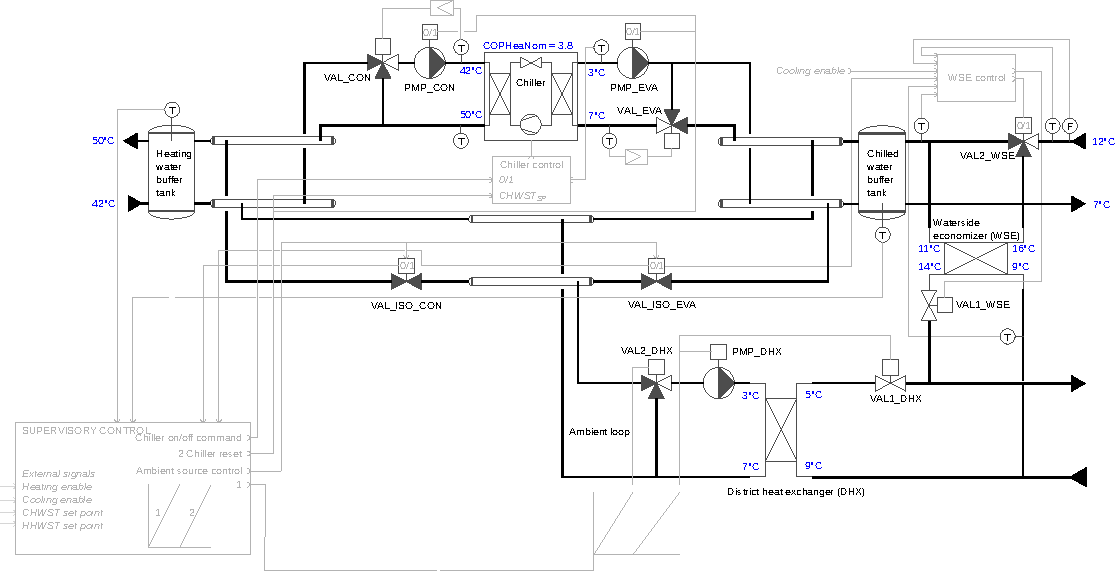
\includegraphics[width=\linewidth]{figures/ChillerBorefield.pdf}
\caption{Schematic of the energy transfer station.}
\label{fig:schematic}
\end{figure*}


\subsection{Demand Signal, Supply Temperature Reset and Secondary Pump Control} \label{sec:demand}

The heating and cooling demand signals are computed based on the maximum control signals of the terminal units: whenever a terminal controller yields a non-zero signal (considering a small hysteresis) the demand signal switches to true.

If there is no demand, the secondary pump is disabled, and the supply temperature is reset to the least extreme value, allowing to operate the chiller at low lift.

If there is a demand, the secondary pump is enabled and its speed is modulated with a PI controller tracking a differential pressure set point at the most remote unit%
\footnote{Modern control sequences~\cite{Llp2019} use a cascade control and reset in sequence the differential pressure set point of the distribution pump (up, first) and the CHW supply temperature set point (down, last) when the number of requests yielded by the terminal units increases---giving the priority to maintaining a low compressor lift over a low pump speed.}%
, and the supply temperature is reset with a PI controller tracking the maximum opening of the control valves of the terminal units to match $90\%$.
We noticed that it is important to reset the controller output so that the design set point value is used when the demand signal switches to true. Otherwise there is a significant delay in satisfying the load, followed by a large overshoot, and the control loop is particularly hard to tune.

\subsection{Central Systems}

\subsubsection{Hydronic Distribution}

The speed of the main distribution pump is modulated with a PI controller tracking a constant pressure differential set point at a remote location. A bypass line is modeled and is sized to recirculate $5\%$ of the design flow rate at the pressure differential set point.

The pump is sized considering no load diversity as the actual diversity observed on the cooling load data (see §\ref{sec:buildings}) is close to $100\%$.

\subsubsection{Geothermal Borefield}

The initial sizing of the borefield is performed based on the method described in \cite{Cline2020}.
The total borehole length $L$ is given by Equation~\ref{eq:sizing}.

\begin{align}
    \label{eq:sizing}
    L &= \frac{\dot{Q}_a R_{10y} + \dot{Q}_m R_{1m} + \dot{Q}_h \left( R_b + F_{sc} R_{6h} \right)}{\left( T_{Ent} + T_{Lvg} \right) / 2 - \left( T_g + T_p \right)}
\end{align}

with

\begin{avec}
    $\dot{Q}_a$ (W): Net annual average heat transfer to the ground, counted positively for heat rejection to the ground%
    \footnote{This is the opposite convention as the one used in \cite{Cline2020}, and Equation~\ref{eq:sizing} is adjusted accordingly.}\\
    $R_{10y}$ (m2.K/W): Effective thermal resistance of the ground computed with a 10-year heat pulse \\
    $\dot{Q}_m$ (W): Net monthly average heat transfer to the ground\\
    $R_{1m}$ (m.K/W): Effective thermal resistance of the ground computed with a 1-month heat pulse \\
    $\dot{Q}_h$ (W): Net 6-hour average heat transfer to the ground\\
    $R_b$ (m.K/W): Borehole overall thermal resistance \\
    $F_{sc} = 0.04$ (-): Correction factor for short-circuit heat losses between the upward and downward flowing legs\\
    $R_{6h}$ (m.K/W): Effective thermal resistance of the ground computed with a 6-hour heat pulse \\
    $T_g$ (C): Undisturbed temperature of the ground \\
    $T_p$ (C): Ground temperature penalty \\
    $T_{Ent}$ (C): Temperature of the liquid entering the borefield \\
    $T_{Lvg}$ (C): Temperature of the liquid leaving the borefield \\
\end{avec}

The effective resistances of the ground are given by the cylindrical heat source formulation from \cite{Carslaw1947} considering a borehole diameter of $150$~mm, a soil conductivity, specific heat capacity, and density of $2.3$~W/m.K, $1000$~J/kg.K, and $2600$~kg/m3, respectively.
This gives: $R_{10y} = 0.17, R_{1m} = 0.15, R_{6h} = 0.08$~m.K/W.
The overall resistance of the borehole is computed based on the method from \cite{Cline2020} considering a double-U tube configuration of DN40 DR 11 HDPE pipes and a grout material with a conductivity of $2.0$~W/m.K. This gives: $Rb = 0.06$~m.K/W.
The hourly load data used for sizing are generated as described in §\ref{sec:buildings}, considering a chiller efficiency of $COP_{Cooling} = 7.0$ in cooling mode (with a condenser entering temperature of $18$°C and an evaporator leaving temperature of $7$°C) and $COP_{Heating} = 4.8$ in heating mode (with an evaporator entering temperature of $7$°C and a condenser leaving temperature of $45$°C).
The central geothermal borefield is designed with a target ground equilibrium temperature of $T_g+ T_p = 12.0$°C, starting from an undisturbed ground temperature of $T_g = 10$°C.
This gives the following required number of boreholes considering a borehole depth of $180$~m.

\begin{align}
    \label{eq:sizing}
    L &= \frac{\dot{Q}_a R_{10y} + \dot{Q}_m R_{1m} + \dot{Q}_h \left( R_b + F_{sc} R_{6h} \right)}{\left( T_{Ent} + T_{Lvg} \right) / 2 - \left( T_g + T_p \right)}
\end{align}


\subsubsection{Cooling Towers}

Discuss sizing and why cooling towers are preferred to dry coolers although they operate mainly in shoulder season at lower humidity ratios (approach of dry coolers is typically higher than 8 K, as opposed to 4 K possible with cooling towers). Is it acceptable to have open towers with regard to the water cleanliness?

\subsection{Modeling Hydronic Systems} \label{sec:balancing}

When integrating the ETS into the whole DHC system model, significant effects of hydronic imbalance were first observed, with the remote ETSs being starved and unable to meet the supply temperature set points, and the ETSs closer to the pump operating at higher flow rates than design.
In addition, convergence issues of the Newton solver appeared, mainly related to the waterside economizer operation.

The first effect was certainly expected using a pressure-driven model of the hydronic system, with no specific care for balancing the connected units. However, and as in real systems, that effect was not expected to disturb the operation to the extent that was observed. Indeed, a controller---controlling for instance a supply temperature or a temperature difference---should limit the primary flow rate under the design values (provided that the primary fluid temperature remains close to the design value). In addition, the heat emission characteristic is supposed to limit the impact of flow shortage, with $50\%$ of the design mass flow rate still providing about $90\%$ of the design heat flow rate for a heat exchanger with $10$ K primary temperature range at design. The only disturbing effects that were expected, and indeed observed, pertain to the low valve authority of the primary control valves that causes control issues, and to the pump speed which is often maxed-out due to the inability to maintain the pressure drop at the remote ETS.

The reason why the ETSs close to the pump often operate at a higher flow rate than design is related to the control based on the heat or cold rejection demand (see §\ref{sec:ets}) that first opens the primary control valve (up to its full opening), then resets down the CHW supply temperature. So the ETSs that are exposed to a higher pressure drop than the design value use the excess flow rate instead of resetting the supply temperature to increase the temperature difference (or rate of heat transfer) with the primary side of the heat exchanger.

Regarding the numerical issues that were encountered we must acknowledge the challenges that remain when modeling closed loop hydronic systems (typically with feedback of a remote diffenrential pressure sensor or of the valve positions to control the main distribution pump).
There has been extensive work that was already carried out to formulate actuator models limiting the size of the DAE systems and exhibiting the proper smoothness required by Newton solvers \cite{Jorissen2015}.
Namely, each actuator model of the Modelica Buildings Library offers the option to solve either for the mass flow rate or for the pressure drop, which breaks the algebraic loop created when two actuators are in parallel or in series, respectively. In addition they provide the option for an additional state variable (mimicking the actuator motion delay) which is another means to avoid an algebraic loop.
In our case, those two modeling features did not solve the convergence issues.

The resolution came from integrating a pressure independent control valve (PICV) into the ETS model to modulate the mass flow rate of the service water through the heat exchangers.
To represent the various technologies of PICVs (dynamic balancing valve in series with a control valve, or built-in flow meter and controller) the model idealizes the physics by solving the simple equation $ \dot{m}_{Act} = u * \dot{m}_{Nom} $, where $u$ is the control signal and $\dot{m}_{Act}$ and $\dot{m}_{Nom}$ are the actual and design mass flow rate, respectively.
The complexity of the model lies in the requirement to properly represent the valve limiting flow characteristics (leakage and full opening) and to compute a pressure drop and a mass flow rate that are continuously differentiable while transitioning between the two characteristics (which is a requirement to apply Newton solvers).
Using that valve model to modulate the service water flow rate offers  key benefits, similar to the ones obtained by the use of PICVs in real hydronic systems.
\begin{enumerate}
    \item The system is dynamically balanced. The primary flow rate can only marginally exceed the design value. Furthermore, this holds true for any operating point, and any location in the distribution network. To the contrary, balancing valves that are commissioned at design conditions may lead to low pressure differences at the boundaries of the control valves close to the distribution pump in the case of closed loop control based on a remote pressure drop sensor and with low demand on the remote valves.
    \item The controllability is optimal. The relationship between the control signal (varying between $0$ and $1$) and the mass flow rate (varying between close to $0$ and close to the design value) is indeed close to linear. To the contrary, with standard control valves, a potentially large range of flow rate variation (spanning beyond the design value) may be mapped to a limited range of variation of the control signal (depending on the valve authority), leading to tedious controller tuning or control instabilities.
\end{enumerate}
In addition, the simulation model is simplified due to the ideal model of the flow rate control loop, for instance when modeling a waterside economizer where the primary valve position is actuated so that the primary mass flow rate equals the chilled water mass flow rate. This eliminates the need for a controller (and for tuning), while reducing the number of state variables and therefore the time to solution, especially for such control loops with fast pressure-driven dynamics.

\section{Application to Resilient Operation Mode} \label{sec:application}

\subsection{Description of the Simulation Experiment} \label{sec:experiment}

\subsubsection{Building Models} \label{sec:buildings}

The original building models are taken from the \href{https://www.energy.gov/eere/buildings/commercial-reference-buildings}{US DOE commercial reference buildings database} and represent new constructions (year 2004) of a medium office, a mid-rise apartment, and a hospital in Chicago IL, USA.
The study focuses on the office building type where resilience metrics are computed based on proxy variables for thermal comfort. The other building types are included to model the load diversity of a typical mixed-use development project.
A multiplier factor of $10$ is applied to the office and apartment types to represent a cluster of similar buildings.
The building models are used in two different ways.

First, simulating those models with EnergyPlus provides heating and cooling load data---the domestic hot water (DHW) loads are not considered in this study---which are used to size the systems.
The resulting building loads are presented Figure~\ref{fig:loads}, the total peak cooling and heating loads are $3.5$ and $3.2$~MW, respectively, and the annual energy is $8.9$ and $5.8$~GWh/y, for a total conditionned floor area of $103,590$~m2.
For the apartment and hospital types, the corresponding time series are then directly used as inputs to the model of the DHC system.
Here, the boundary of the Modelica model is the load side of the ETS component where the building loads are converted into a mass flow rate and temperature variation with an interface component approximating the emission/flow rate characteristic of the building HVAC system.

Second, for the office type, the EnergyPlus input data file is consumed to generate an FMU for Model Exchange that can be coupled to a Modelica model using the Spawn of EnergyPlus toolchain \cite{Wetter2020}. Here, the boundary of the Modelica model encompasses the building HVAC system as well as the air volume of the rooms, while the building envelope is modeled with EnergyPlus.
The building HVAC system is a variable air volume (VAV) system with hot water reheat.
The system components are sized based on the peak loads computed with EnergyPlus (with a cooling load diversity factor of $0.7$) and the requirements from \cite{ASHRAE62.1} for ventilation parameters and from \cite{ASHRAE90.1} for other limiting operating conditions.
The control sequence is adapted from \cite{ASHRAE2006}.
The main features of the implementation are described in \cite{Wetter2022}, and some refactoring was carried out mainly for scalability (with $15$ conditioned zones plus $3$ plenum zones where the air return inlets are located) and to expose all sizing parameters in a central parameter record. However, some limitations from the original model pertain and call for caution and consolidation efforts for large multi-zone applications, namely: the model represents a single supply fan system with no return fan; the parametrization of the duct network is representative of a non-ducted return systems; there is no space static pressure control (unrealistic pressure values are indeed observed at high flow rate and low exhaust damper opening); the fan and motor efficiency is constant.

\begin{figure*}[!htbp]
    \centering
    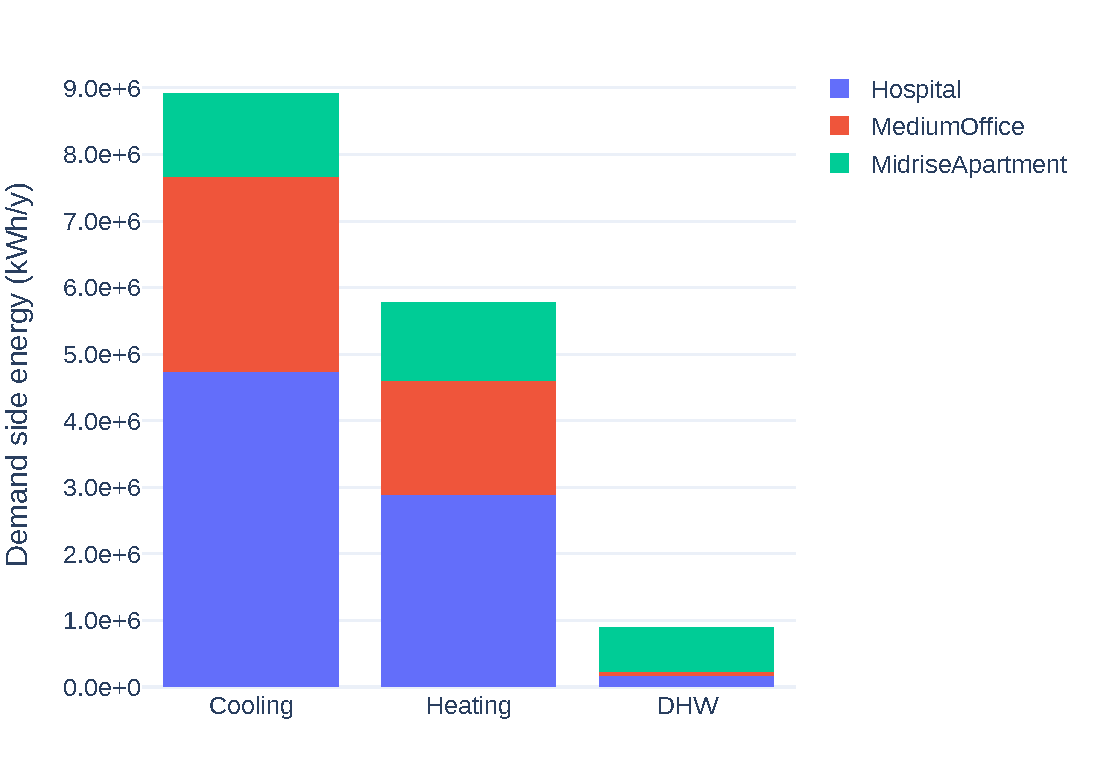
\includegraphics[width=.7\linewidth]{figures/LoadsSum.pdf}
    \caption{Building loads computed with EnergyPlus, integrated over the year, including the multiplier factors used to represent clusters of similar buildings (DHW loads are presented for reference but are not considered in this study).}
    \label{fig:loads}
\end{figure*}

\subsubsection{Weather Data} \label{sec:weather}

The weather data for annual simulation is the TMY3 weather file for Chicago IL, USA.
A so-called "resilience design day" is generated based on the most severe conditions in July from that TMY3 weather file, which happen to be more conservative than a design day generated based on the method proposed in \cite{ASHRAE2017} Chapter 14 considering the annual $0.4\%$ design dry-bulb temperature and the mean coincident wet-bulb temperature.
During the resilience design day the dry-bulb temperature range is $[23.3, 35.0]$~(C), the wet-bulb temperature range is $[22.5, 26.9]$~(C), and the global horizontal irradiance peaks at $931$~W/m2.
The resilience design day is repeated $7$ times during the month of July to generate a "resilience design week" over which the comfort analysis is performed.

\subsubsection{Internal Heat Gains} \label{sec:gains}



\subsection{Results} \label{sec:results}

Discuss impact on peak and average power and lost hours of operation

\subsubsection{Base Case} \label{sec:base}


\subsubsection{Sensitivity Analysis} \label{sec:sensitivity}

Building HVAC System

\begin{figure*}[!htbp]
\centering
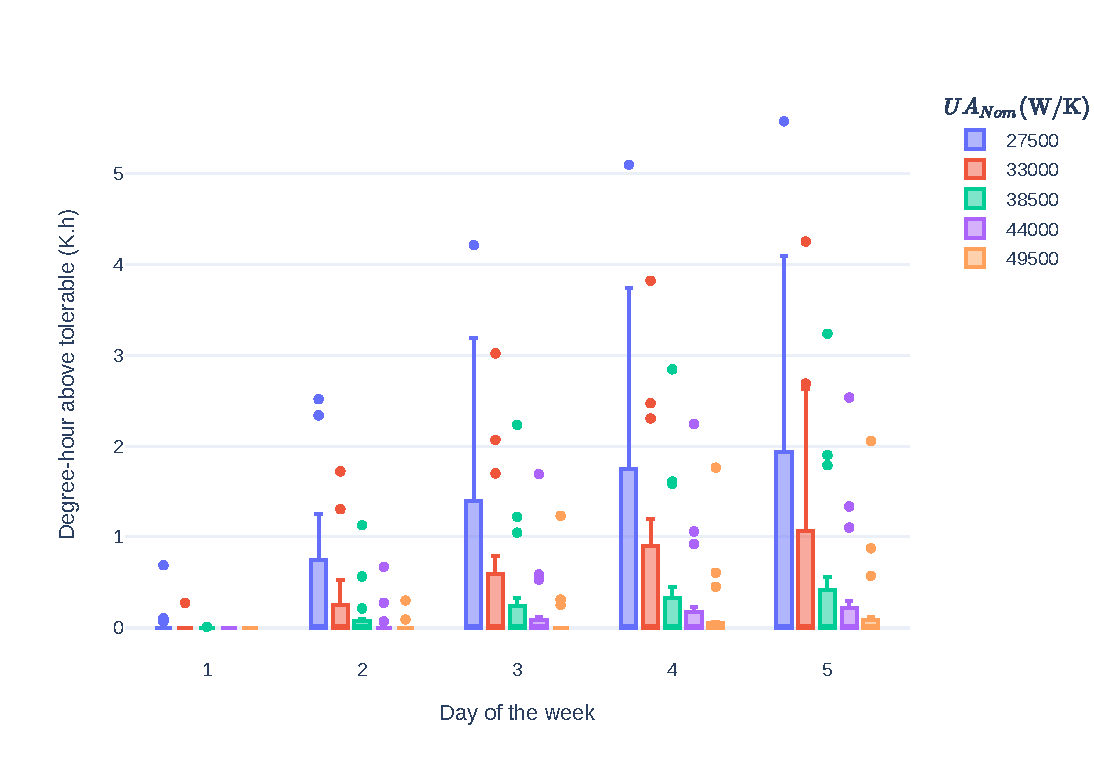
\includegraphics[width=\linewidth]{figures/CoilSizing.pdf}
\caption{Sensitivity to the cooling coil sizing.}
\label{fig:coil}
\end{figure*}

\begin{figure*}[!htbp]
\centering
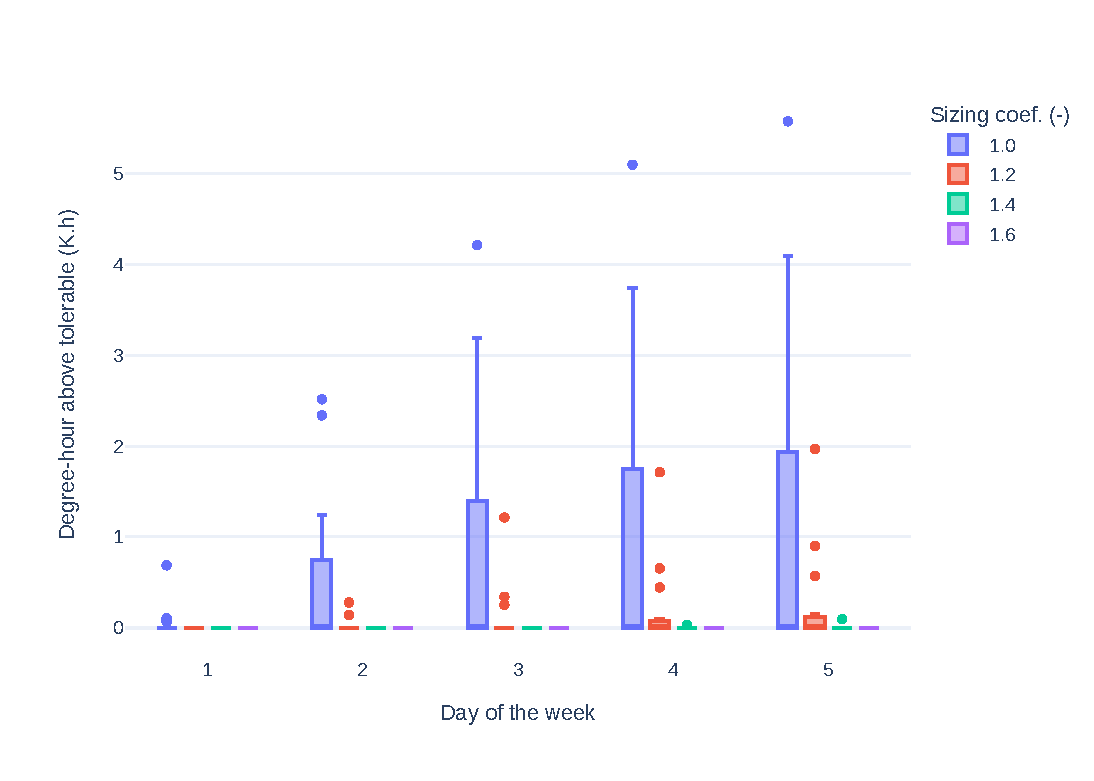
\includegraphics[width=\linewidth]{figures/FanSizing.pdf}
\caption{Sensitivity to the fan sizing coefficient.}
\label{fig:fan}
\end{figure*}

District Central Systems

\begin{figure*}[!htbp]
\centering
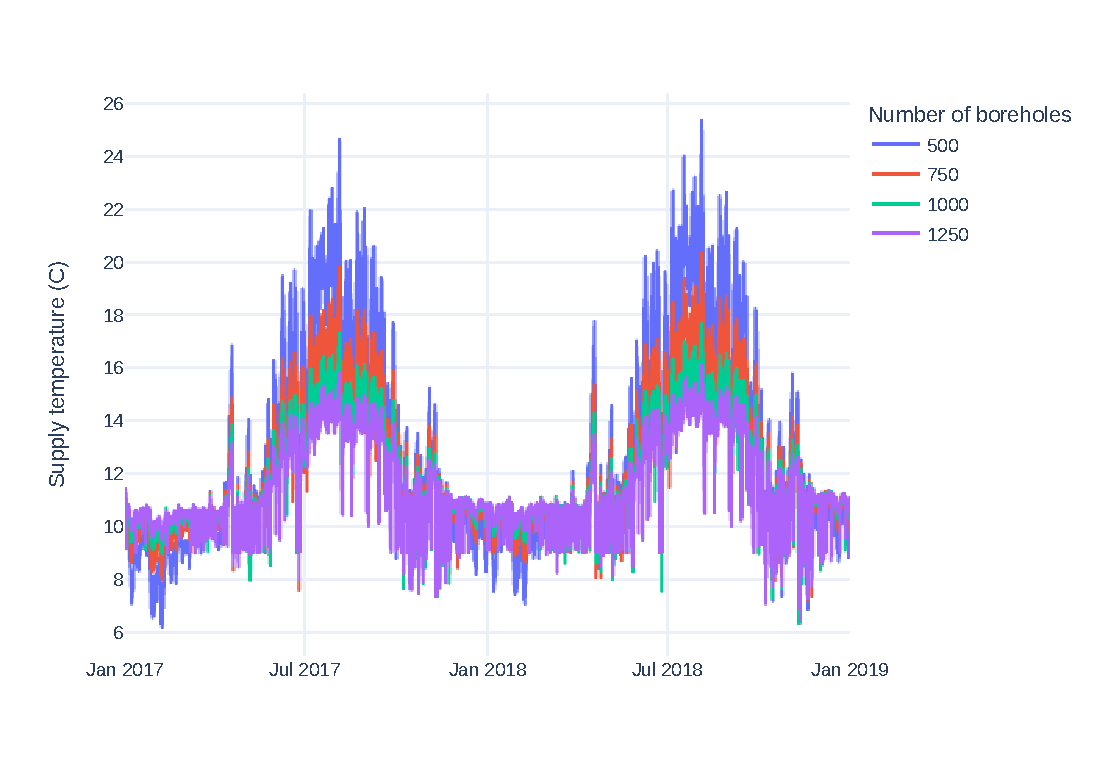
\includegraphics[width=\linewidth]{figures/GeoSizing.pdf}
\caption{Sensitivity to the geothermal borefield sizing - District water supply temperature.}
\label{fig:geo_sizing}
\end{figure*}

\begin{figure*}[!htbp]
\centering
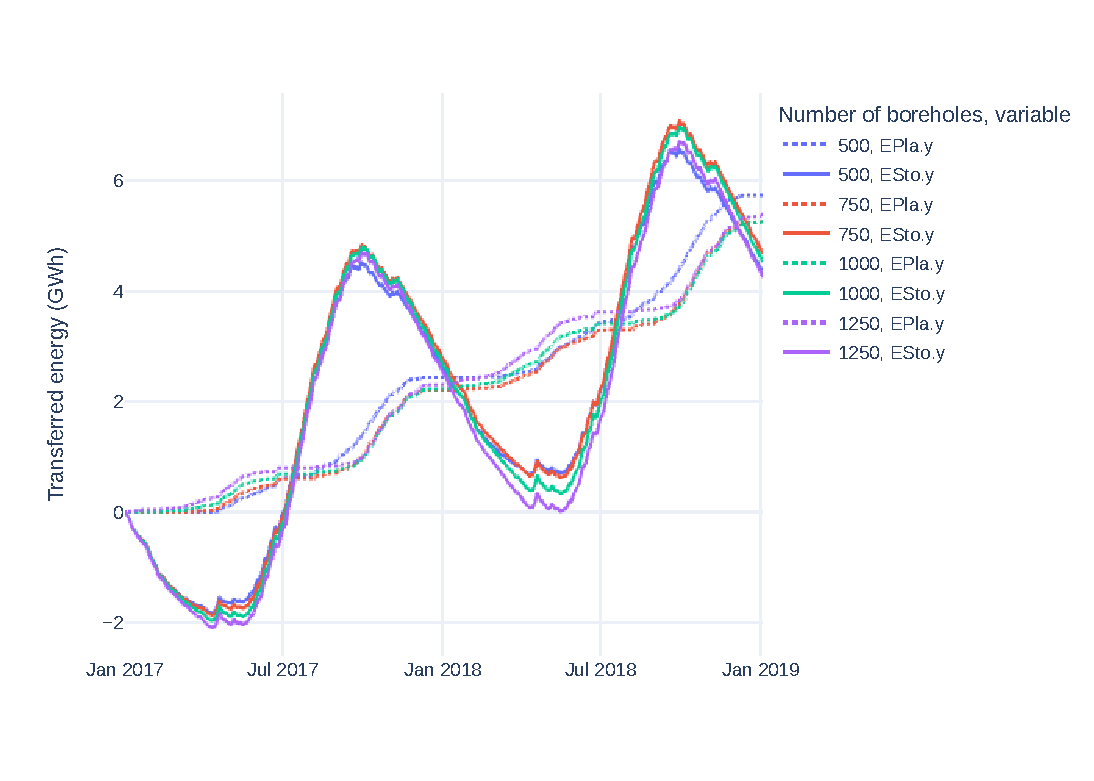
\includegraphics[width=\linewidth]{figures/GeoSizingE.pdf}
\caption{Sensitivity to the geothermal borefield sizing - Energy transferred from the district loop through the borefield ($ESto.y$) and through the cooling towers ($EPla.y$).}
\label{fig:geo_cooling}
\end{figure*}


\begin{figure*}[!htbp]
\centering
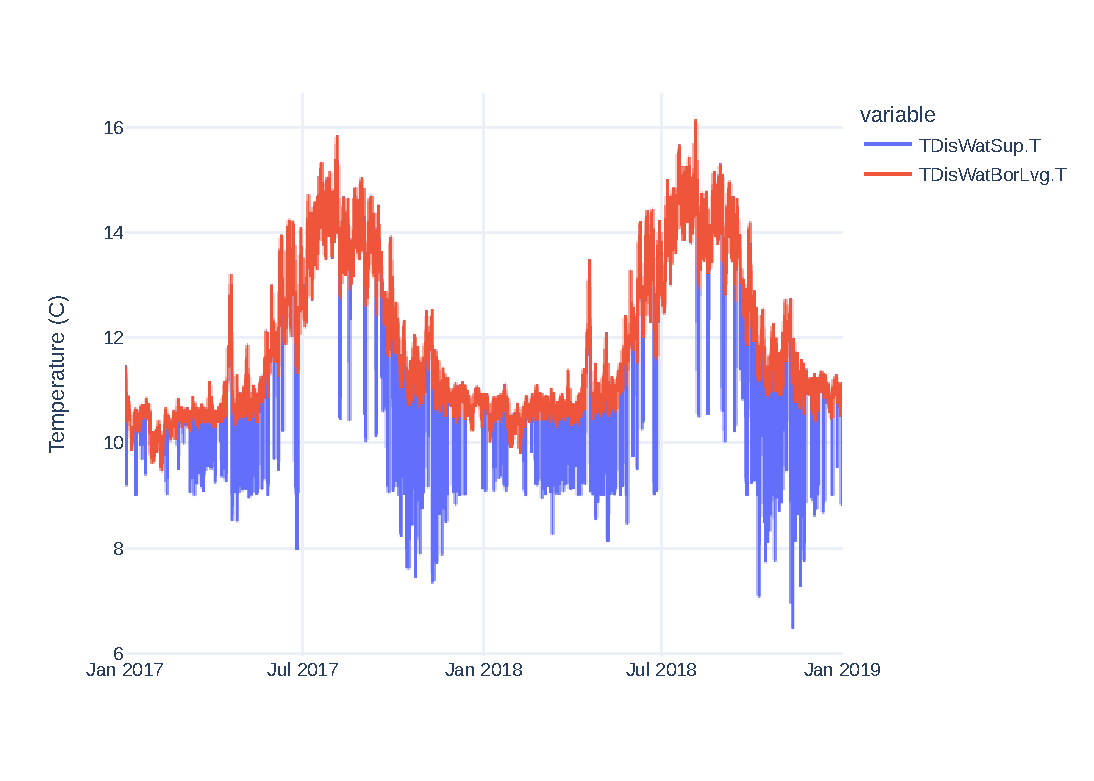
\includegraphics[width=\linewidth]{figures/GeoBestCaseT.pdf}
\caption{Illustration of the cooling towers effect on the case with 1250 boreholes - District water supply temperature ($TDisWatSup.T$) and borefield leaving temperature ($TDisWatBorLvg.T$).}
\label{fig:coolingeffect}
\end{figure*}


\subsubsection{Impact on Energy Use} \label{sec:energy}

Waterside Economizer







\section{Conclusion} \label{sec:concl}


Future studies should investigate the benefits of source-side to source-side connection (indirect heat recovery at lower lift) as opposed to direct heat recovery at higher lift.

\section{Acknowledgements} \label{sec:acknowledge}
